\chapter{引言}
\label{cha:intro}


\section{研究背景与意义}

自Web2.0普及后,大量网民每天在互联网生产着不同媒体类型的数据,其中包含各种信息,如个人生活经历,购买行为,对产品服务的体验评价,对社会时事的看法等等。从人们的日常社交需求来看,这种借由互联网媒体的分享非常便捷,我们可以了解到亲朋好友的近况,也或者随时和不认识的网民交流对具体事件的想法。在商业上,借由对用户的网络行为进行分析,企业可以对应客户或者潜在客户有更深入的了解,对他们的需求和反馈及时作出反应将带来战略性的优势。在社会管理上,政府可以透过对网民在网络上的发言了解人民的想法和舆论的走向,进而作出相应的措施。正因为互联网的普及,才使得以上基于对特定人群的了解来进行决策的做法成为可能。随着数据资源变得丰富,相应的技术在近年有明显的发展,目前市面上已经有公司(如国内的腾讯和阿里巴巴,以及国外的微软和亚马逊等)提供基于大型社交媒体平台(如微博,讨论区等)上的数据进行意图分析相关的规泛化服务,然而相应的技术依然有进步空间,研究工作还在不同方向上摸索。

情感在人们的思想表达和交流中起着重要作用\cite{Banerjee2015Detection},比起了解该思想的细节内容,情感对应该思想的大体倾向。譬如在分析用户对新产品的评论时,从对正负性情感反馈的统计可以得知新产品是否能让大部分的客户满意,或者筛选出表示不满意的用户再进行深入分析,因此情感识别是意图分析中属于非常重要的一环。而由于在互联网上,大部分情况下用户以文本表达想法,面向文本的意图识别成为了近年的最要研究课题之一。相对于人们面对面交流的场景,聆听者可以根据发言者的肢体语言,面部表情以及声调变化等额外提示更好地理解发言者所表达的内容,然而这些信息并不存在于文本当中,这也正是对文本进行情感识别本身的难点之一\cite{SemEval2019Task3}。

反讽的修辞手法在意图识别当中起着特殊的影响。Henry Watson Fowler在《The King's English》一书中描述“即使对反讽的定义有数百种, 其中只有包含'表面意思和实际意思不同'这个概念的才能被接受”。Eric Partridge 在《Usage and Abusage》一书中指出“反讽存在于所表达意思的另一面”。总的多说当反讽在文本中出现,那么文本所表达的意思应该和字面表达的意思完全相反。譬如某人表示“我就喜欢你不断挑战我的底线”,从字面上理解应倾向于正面情感,然而根据常识可知“挑战底线”是一种让人反感的行为,与“喜欢”相矛盾。这段文字实则暗示发言者的“底线”正被“你”“挑战”,表达的是负面情感。因此在意图识别和情感分析当中,正确检查出反讽的使用能够避免对内容的错误理解。

\section{国内外研究现状}

\subsection{情感模型}

情感计算的基础是对情感作出描述,现有的描述方式可以分成两个大类: 范畴观和维度观。范畴观即把不同情感对应到一组离散的情感标签上Alm等人\cite{Alm2005Emotions},其中具代表性的有Plutchik的情感模型\cite{Plutchik1980Emo}和Ekan的情感理论\cite{Ekman1992An}和。Plutchik的情感模型包含十种情感:愤怒、恐惧、悲伤、厌恶、期待、信任、高兴、惊讶;这些情感都各自对应具有重要生存意义的行为,各种复杂的情感都是由这此基本情感构成,另外这十种情感可以分成五组对立的情感对。Ekan在十年后提出的情感理论和Plutchik的相似,但相对地少了期待和信任,是一个六类情感模型。

\begin{figure}[h]
  \centering%
  \subcaptionbox{三维模型\label{fig:plutchik_emotion_wheel_3d}} %[3cm] 标题的长度,超过则会换行,如下一个小图。
    {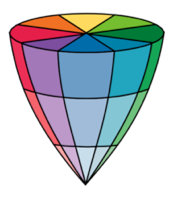
\includegraphics[height=4cm]{img/plutchik_3d.png}}%
  \hspace{4em}%
  \subcaptionbox{二维模型\label{fig:plutchik_emotion_wheel_2d}}
      {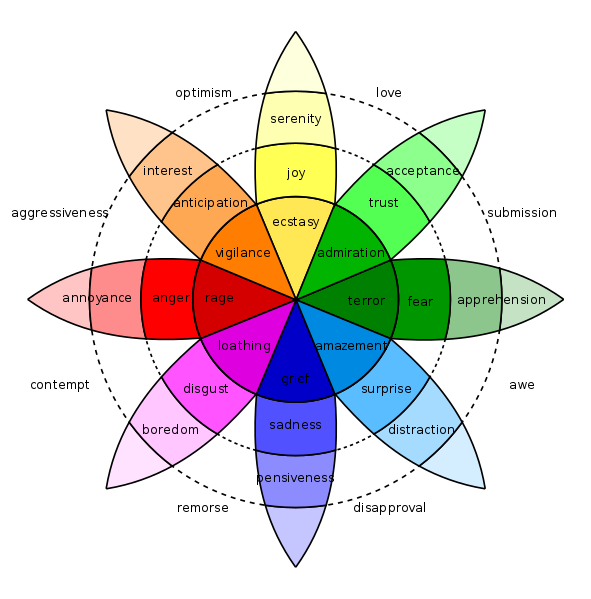
\includegraphics[height=8cm]{img/plutchik_2d.png}}
  \caption{Plutchik\cite{Plutchik1980Emo}提出的情感轮模型}
  \label{fig:plutchik_emotion_wheel}
\end{figure}

以维度观描述情感就是把情感映射到多维空间的点上,而目前维度观情感模型以二维和三维空间的为主。二维情感模型中较有代表性的是Russell提出的环状模型(Circumplex Model)\cite{Russell1980Cir} ,其中纵坐标对应情感的激活度(Arousal),横坐标对应情感向性(Valence),而不同的情感则分布在一个环状的区域内。Bradley等人\cite{Bradley1992Rem}提出的向量模型(Vector Model)对横轴和纵轴的定义相似,但其理论认假设高激活度的情感应该有较明显的正向或负向,相对地低激活度的情感则偏向中性,故情感分布在一个回力标形状的区域。Watson和Tellegen \cite{Watson1985Tow} 提出的 PANA(positive activiation-negative activation)模型和前两者在理论基础上则有明显的不同,他们认为情感的正面作面和负面作用是两个独立的成分,所以在模型中纵轴和横轴分别表示情感正面作用和负面作用的强弱,其效果相当于把Russell等人提出的环状模型的向量空间旋转45度\cite{Rubin2009A}。

基于三维空间的情感模型中具有代表性的有Plutchik\cite{Plutchik1980Emo}提出的情感轮模型,Plutchik认为情绪之间包含强度,相似性和两极性三种维度,椎体的顶部和底部分别对应强的情绪和弱的情绪,相似的情感对应椎本中相近的位置,对立的的情绪则会对应到椎体中对立的位置上。另外还有Mehrabian \cite{Mehrabian1996Pleasure}提出的PAD模型,其三维空间的三个坐标轴分别对应情感愉悦度(Pleasure)、激活度(Arousal)以及优势度(Dominance)。较近期被提出的是Hugo\cite{Hugo2012A}的情感立方体模型,其三维空间的三个坐标轴分别对应5-羟色胺(5-hydroxytryptamine, 5-HT), 多巴胺(dopamine,DA)和去甲肾上腺素(noradrenaline,NE)三种神经递质所产生信号的强弱,并对空间中一个立方体的八个顶点标记了其对应的情感。

\begin{figure}[H] % use float package if you want it here
  \centering
  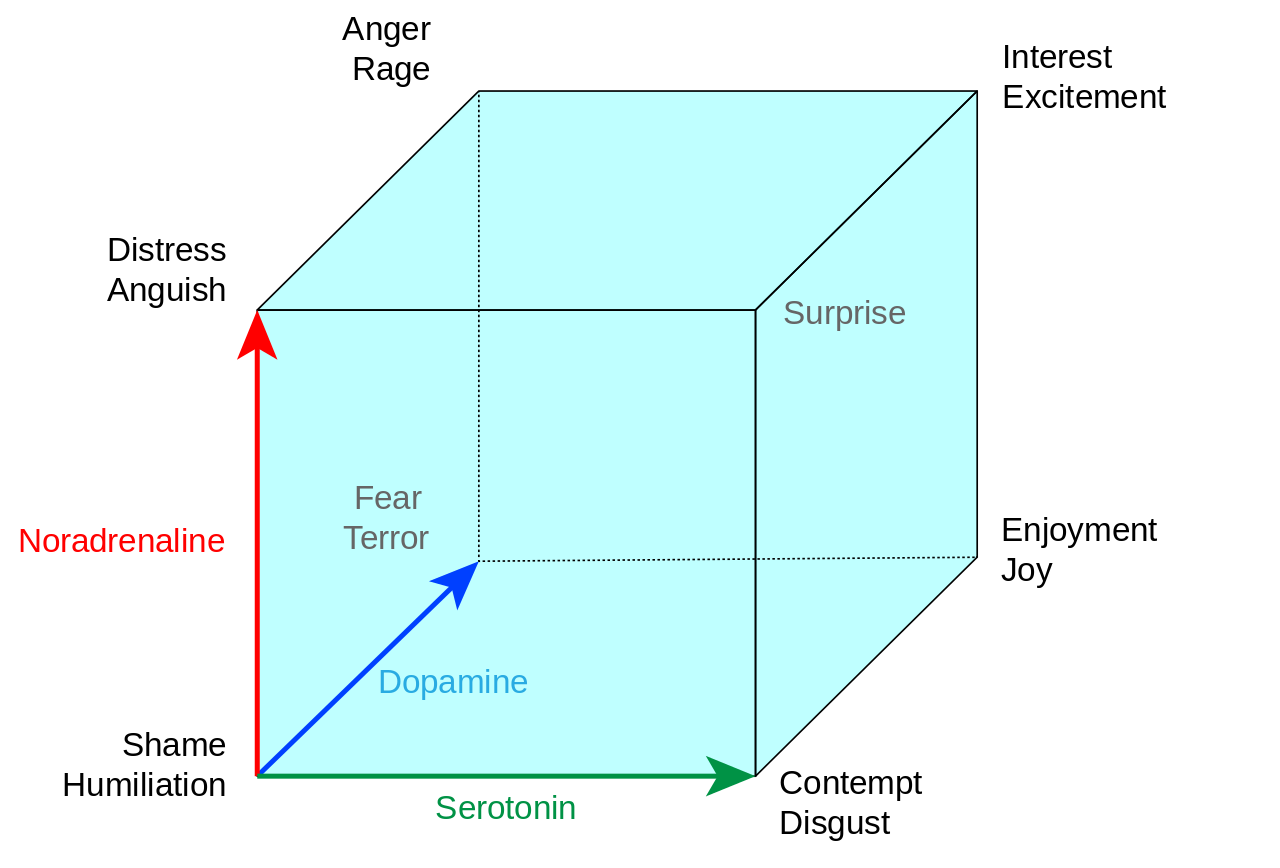
\includegraphics[width=0.8\textwidth]{img/hugo_cube_of_emotion.png}
  \caption{Hugo\cite{Hugo2012A}的情感立方体模型}
  \label{fig:hugo_cube_of_emotion}
\end{figure}


\subsection{情感识别}

对应上述情感模型的分类,情感识别研究可以分成两类。第一类对应范畴观,给定一组情感类型,判断一段文本或针对文本内的某个方面所表达的情感倾向于该组情感中的哪一个,或者是否包含这一组情感中的一个或多个情感。如国际比赛SemEval2018 \cite{mohammad2018semeval}任务一的子任务要求识别一段微博中是否包含愤怒、恐惧、悲伤等十一种情感中的一种或多种情感。另一类情感识别研究对应维度观,对于给定的情感属性,判断一段文本中该情感属性的强度。其中常见的有情感向性的二分类问题(正性或负性)、三分类问题(正性、中性或负性)、五分类问题(非常正性,正性、中性、负性或非常负性)。其中五分类问题的研究对象一般是互联网上五星评分制的产品评论或者电影评论等。而对目前文本情感识别的研究按照文本的粒度可以大致分成三类:文章级别, 句子级别,属性级别。

在文章级别的情感识别中,虽然一篇文章由多个句子组成,均假设其整体存在某种情感偏向,而研究目标则是自动识别出该种情感偏向的类型或强度。Turney \cite{turney2002thumbs} 利用线上电影评论中"推荐"(大拇指朝上)和"不推荐"(大拇指朝下)的标记研究对电影评论的正负性情感识别。他提出利用点互信息(Pointwise Mutual Information,PMI)来评估单词的语义倾向性,其中PMI透过在大型语料库中统计两个单词的共同出现的情况来评估两个单词的相似度。首先利用PMI值评估各个单词与正向情感的代表性单词"excellent"和负向情感的代表性单词"poor"的相似性,再取这两个PMI值作差得出该单词在语义上倾向于哪一种情感。最近透过计算整段评论的平均语义倾向性评估整体的情感倾向。Pang和Lee \cite{pang2004sentimental} 采用了不同的方法研究相同的问题。他们首先对评论中每个句子的主观程度进行评分,利用评分构造一个带权重的句子关系图,再基于最小割算法结合上下文加强对每个句子主观程度的判断,过滤评论中不带主观情感的句子后再判断整个评论的情感向性,以此加增强了识别能力。

然而一篇文章有可能同时表达了多种观点和情感,因此有另一类研究针对句子或短文本所表达的情感,即句子级别的情感识别。由于句子的文本长度较文章的短,文本内部的逻辑较简单,但相对地所包含的提示信息也较少,课题的难点与前者有所不同。Khan等人 \cite{khan2011sentiment} 研究了对线上评论中句子进行正负性情感识别。他们首先区分出评论中各个句子的主观性和客观性,然后针对带主观情感的句子,利用开源自然语言工具SentiWordNet获取各个单词的正负情感属性,再根据句子的词性标注和他们设计的规则计算整个句子的情感向性。他们的研究默认单词的正负情感属性在不同场景下不变,然而Li等人\cite{li2013constructing} 指出部分单词在特定场景下会有不同的情感向性,因此他们提出了一种有监督学习方法,自动学习各单词在指定领域下的情感向性,以此作为文本的特征,并应用于对产品评论的情感识别中。实验结果显示使用SentiWordNet提供的全局情感评分和针对领域评估的情感评分相比,后者的识别性能力更好,同时验证了他们的假设。

在一些应用场景当中,我们希望了解发言者对某个特定对象或者它的某个特定属性的想法。譬如新手机推出市场后,厂商需要了解用户对手机的续航能力,拍照质量,交互体验等各方面的评价,对于评论中同时谈论手机的多个方面并且好评和差评不一时,应该针对各个属性分别识别发言者所表达的感情,因此有了属性级别的情感识别。Che等人 \cite{che2015sentence} 提出一种句子压缩算法,透过对句子进行依存句法分析,过滤与目标属性的情感无关的内容。他们采用了多种语义和语法特征作为输入,以条件随机场(Conditional random field,CRF)作为分类器。实验结果显示过滤掉不相关的文本部分后,识别性能有所提升。

Wang等人 \cite{wang2016attention}研究了对网上评论中特定实体或属性的情感识别。他们提出了一个基于注意力机制的长短期记忆网络(Long Short-Term Memory,LSTM),特点在于只以词向量作为输入,而不采用其他传统的语义和语法特征,另外利用注意力机制自动识别与目标相关的内容。他们实验基于国际比赛SemEval-2014任务四中的一个子任务,结果然显示他们的系统性能达到了当时的技术水平。另外经过注意力单元的输出进行分析,验证了注意力机制能有效识别文本中与目标相关的内容。

\subsection{反讽识别}

反讽识别技术作为很多自然语言系统的一部分,其应用场景有线上评论分析,人机对话等,对正确理解评论的情感倾向和话语的意图起着辅助的作用。Tsur等人 \cite{tsur2010icwsm} \cite{davidov2010semi}研究了对微博平台Twitter上的微博以及电商平台亚马逊上的评论进行反讽强度的识别,按明显不含反讽和明显表示反讽分成五级,由人工进行标注。他们提出的SASI算法分别从文本提取了词频相关的模式特征以及基于标点符号的特征,以K最近邻算法作为分类器。另外利用在Twitter按井号标签\#sarcastic自动爬取了额外的反讽语料用于初步的模型训练。对实验结果的比较证明了各种特征的有效性以及添加额外语料对模型训练的帮助。

为了以较低成本获取大量的反讽语料,很多研究从微博平台根据井号标签自动筛选出可能带反讽的微博。Reyes等人 \cite{reyes2013multidimensional} 利用\#irony,\#education, \#humor, \#politics在Twitter上自动获取四组英语微博,并把\#irony对应的微博和另外三组微博两两组成二分类实验。他们提出了四个方面的文本特征以及对应的提取方法,包括:特殊标记(词汇和标点符号等)、不可预期性、表达风格、情感特性;并比较了每项特征在各组微博中的出现情况,显示了与反讽类微博的相关性。另外分别采用朴素贝叶斯和决策树作为分类器,但没有明显的性能区别。

类似的数据收集方法对其他语言同样适用。Kunneman等人\cite{kunneman2015signaling}则利用对应的德语井号标签来获取反讽语料,以此研究德语微博中的反讽识别。他们取N元语法作为输入特征,以Balanced Winnow \cite{littlestone1988learning}作为分类器,在测试集上达到约0.85的召回率和0.87的AUC值。但他们进一步经过人工检验评估了基于井号标签自动标注的有效性,分析结果显示该方法获取的反讽样本中包含约10%的躁声。

有别于早期以手动设计的特征作为输入和以非神经网络的机器学习方法建模,Poria等人 \cite{poria2016deeper} 首次将神经网络应用于对微博的反讽识别。他们的算法框架主要包含四个卷积神经网络,并分别利用不同的数据集进行预训练,分别对应反讽识别、情感极性识别、情感类型识别和性格识别。最后取四个卷积神经网络的中间结果作为特征,利用支持向量机(Support Vector Machine, SVM)进行后融后得出最终预测结果。实验显示引入反讽识别以外的三个语料库提升了系统的识别能力。


\section{研究内容和贡献}

pass

\section{本论文的内容安排}

pass
